\chapter{ORB-SLAM在家居设计和增强现实中的应用构想}

\section{ORB-SLAM方法简述}

ORB-SLAM \cite{Mur-Artal2015}
是近几年比较火热的单目相机的SLAM方法,它在PTAM的基础上采用了效率更高的特征提取和优化算法,改进了PTAM的双进程为三进程,加入闭环检测(loop closing),并优化了代码结构,使得该算法较PTAM更稳定,更实用,也更有移植到移动端的潜力。

该算法的流程如\autoref*{fig:ORBprocess}所示,算法主要维护三个进程:追踪进程(Tracking)与PTAM类似,主要用于相机姿态的估计,但不同的是采用了比FAST更优的ORB \cite{Strasdat2011}
特征点提取方法,同时改进了关键帧的判定。局部映射进程(Local Mapping)则与PTAM中的映射进程类似,在有了新的关键帧之后,算法需要维护关键帧集合,构建重建信息,同时进行BA优化。ORB-SLAM算法维护的第三个进程,即闭环检测进程(loop closing),利用了DBoW2\cite{Galvez-Lopez2012}技术,通过构建词典检测图片序列中的语义场景,从而判定相机轨迹中是否存在闭路的情形,
同时对检测到的闭路进行优化,提高追踪精度并减少重复计算。

为了降低全局的时间复杂度,ORB-SLAM维护一个基于关键帧到关键帧的图结构(Covisibility Graph)
\cite{Galvez-Lopez2012}
,用图模型中边的权值(共享特征点数量)衡量关键帧的相似度,同时取稠密图中的MST(Essential Graph)作为子图实际参与优化,在保证鲁棒性的前提下尽可能提高效率。


\begin{figure}[!htbp]
\centering
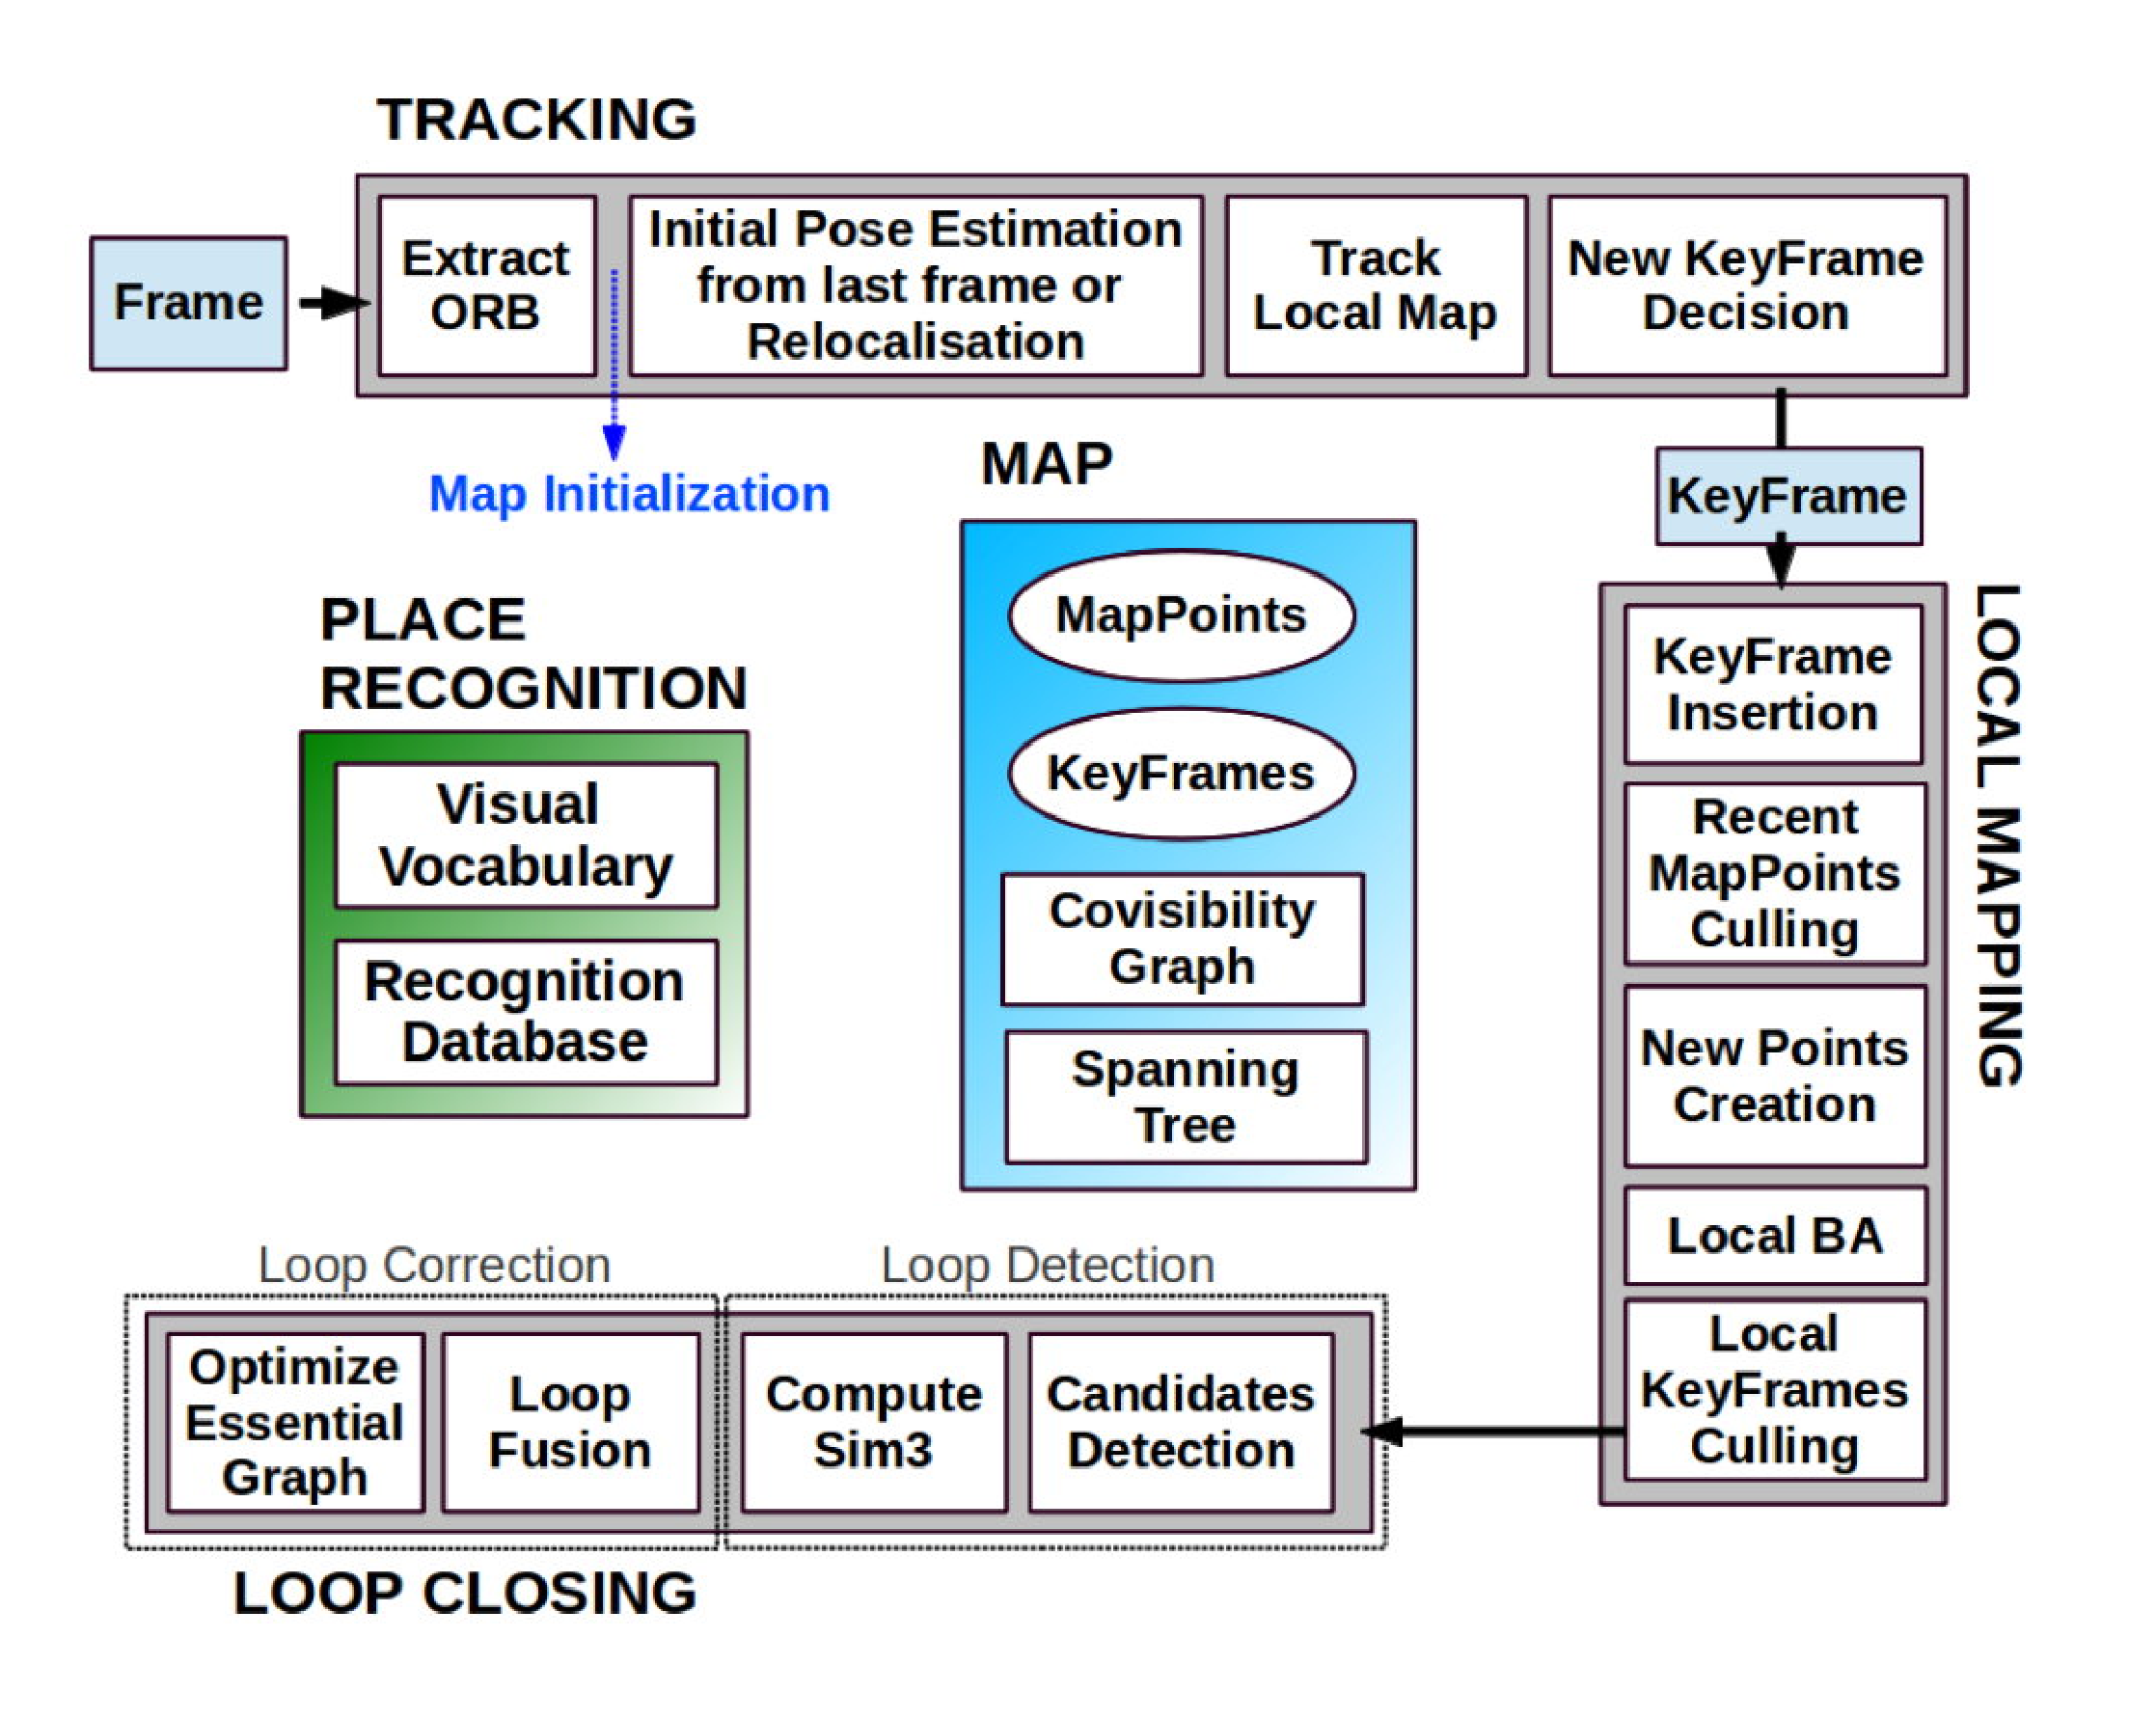
\includegraphics[width=12cm]{ORBSLAM.pdf}
\caption{ORB-SLAM算法的主要流程示意}
\label{fig:ORBprocess}
\end{figure}

\section{ORB-SLAM方法评价}
ORB-SLAM基本延续了 PTAM 的算法框架,但对框架中的大部分组件都做了改进, 归纳起来主要有 4 点: \cite{刘浩敏2016基于单目视觉的同时定位与地图构建方法综述}

(1)ORB-SLAM选用了ORB特征,基于ORB描述量的特征匹配和重定位,都比PTAM具有更好的视角不变性。此外,新增三维点的特征匹配效率更高,因此能更及时地扩展场景。扩展场景及时与否决定了后续帧是否能稳定跟踪。

(2)ORBSLAM加入了循环回路的检测和闭合机制, 以消除误差累积. 系统采用与重定位相同的方法来检测回路(匹配回路两侧关键帧上的公共点),通过方位图(Pose Graph)优化来闭合回路。

(3)PTAM需要用户指定2帧来初始化系统,2帧间既要有足够的公共点,又要有足够的平移量。平移运动为这些公共点提供视差(Parallax),只有足够的视差才能三角化出精确的三维位置。ORB-SLAM 通过检测视差来自动选择初始化的2帧。

(4)PTAM扩展场景时也要求新加入的关键帧提供足够的视差,导致场景往往难以扩展。ORB-SLAM采用一种更鲁棒的关键帧和三维点的选择机制——先用宽松的判断条件尽可能及时地加入新的关键帧和三维点,以保证后续帧的鲁棒跟踪,再用严格的判断条件删除冗余的关键帧和不稳定的三维点, 以保证 BA 的效率和精度。

总之,ORB在理论开创性方面远不及PTAM,然而ORB也绝不仅仅是PTAM添加了loop closure模块并替换图像特征为ORB而已。它吸收了近几年monoslam领域的很多理论成果,比如逆深度的使用,g2o工具箱的优化等。

但是ORB-SLAM相较于PTAM算法来说,它的效果已经比PTAM好多了,\autoref{fig:ORBSLAM2}和\autoref{fig:ORBSLAM3}就是我们实际运行ORB-SLAM得到的效果图。可以发现无论是在稳定性和重建规模,以及对于闭环的检测上,ORB-SLAM都优于PTAM,有了一个非常显著的改进。

\begin{figure}[!htbp]
\centering
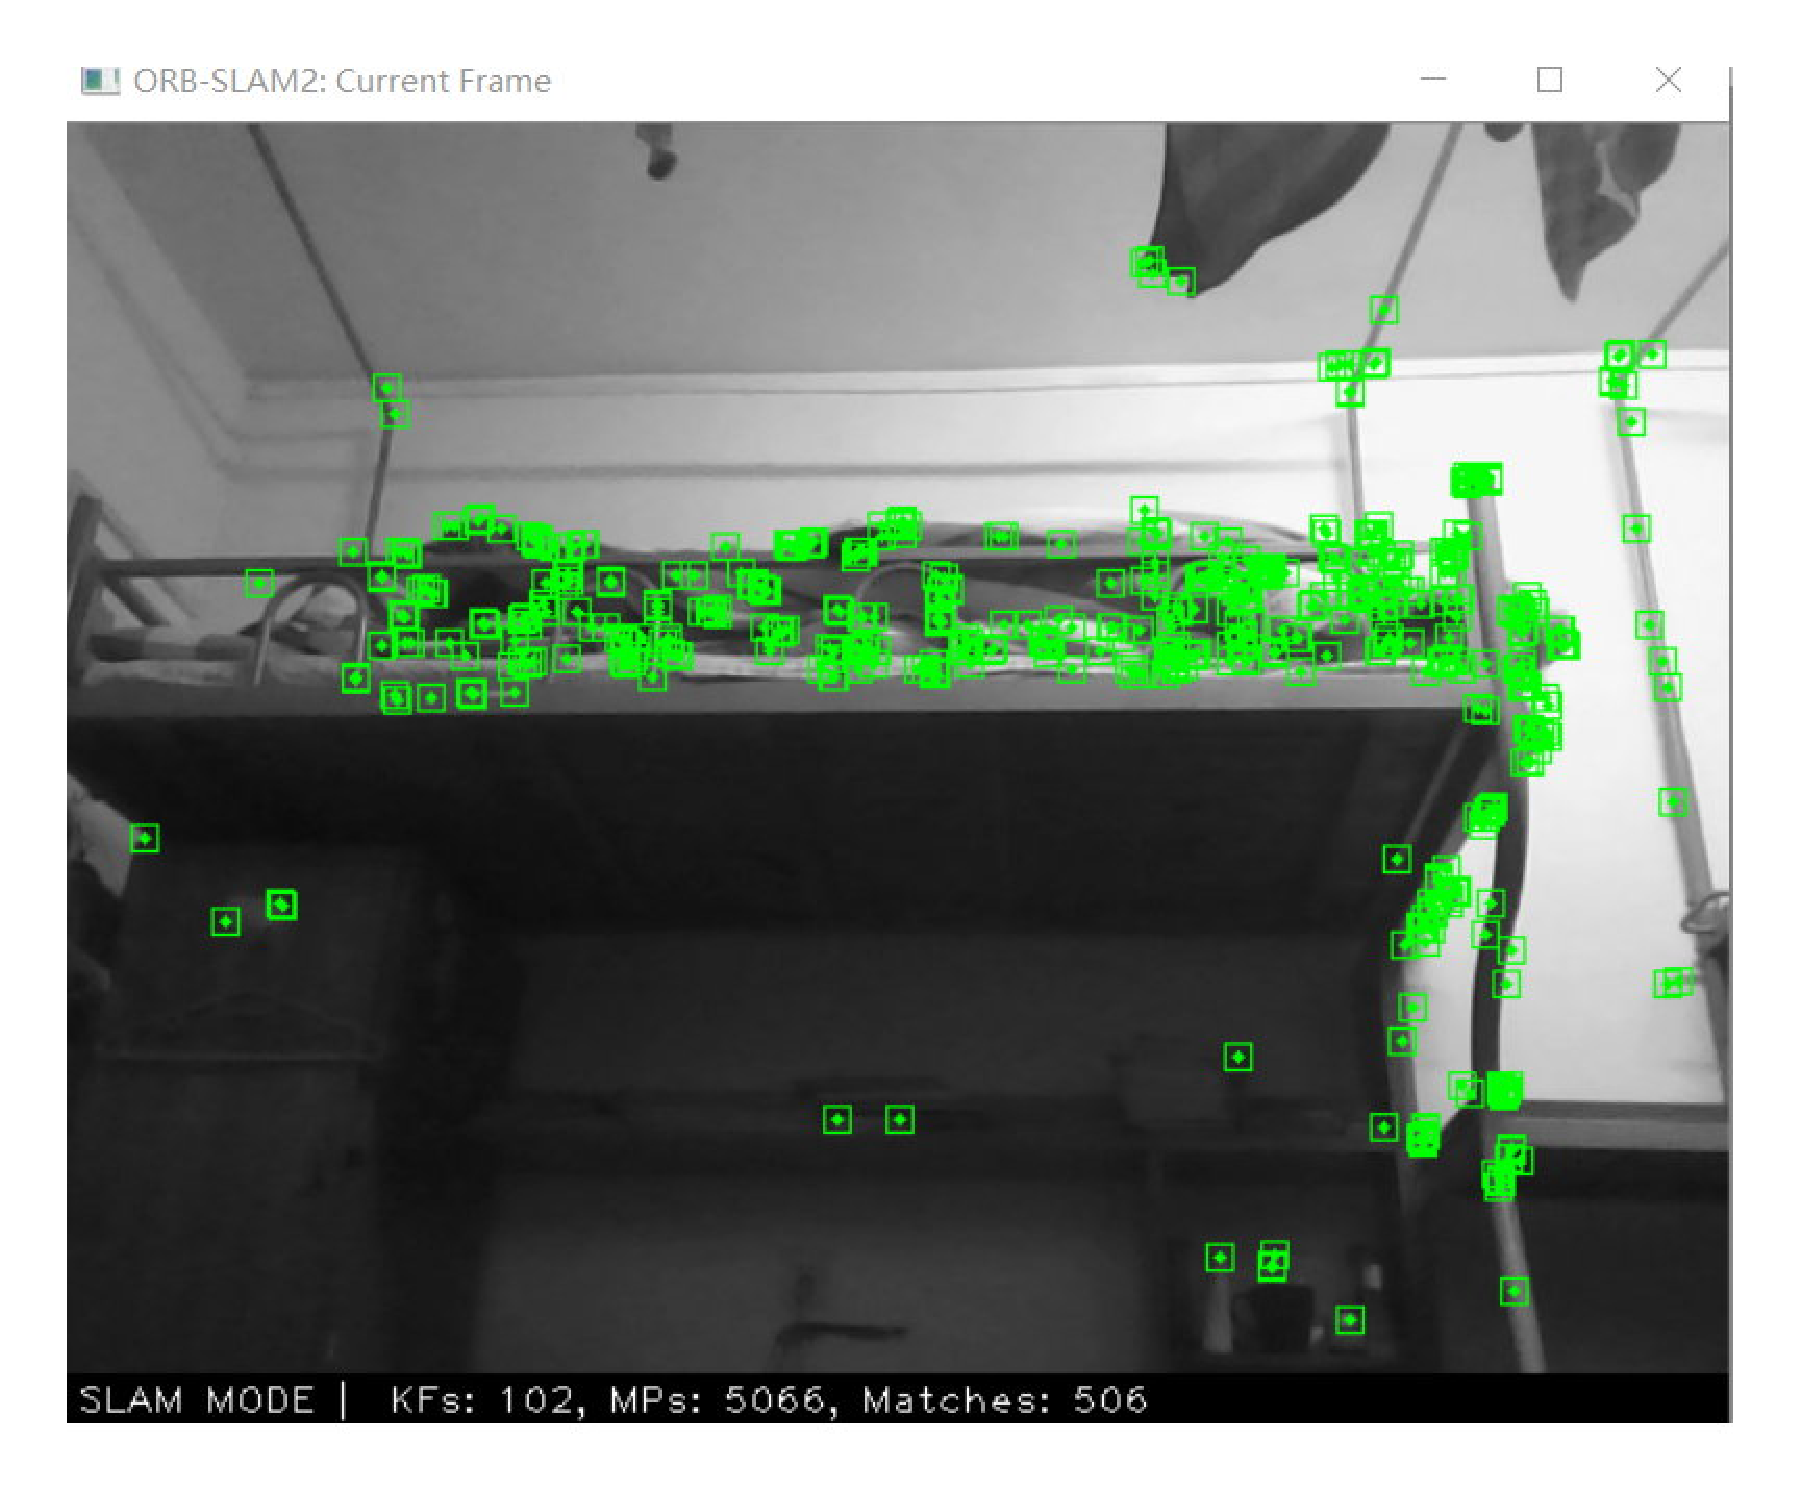
\includegraphics[width=10cm]{ORBSLAM1.pdf}
\caption{ORB-SLAM实际关键帧检测示意}
\label{fig:ORBSLAM2}
\end{figure}
\begin{figure}[!htbp]
\centering
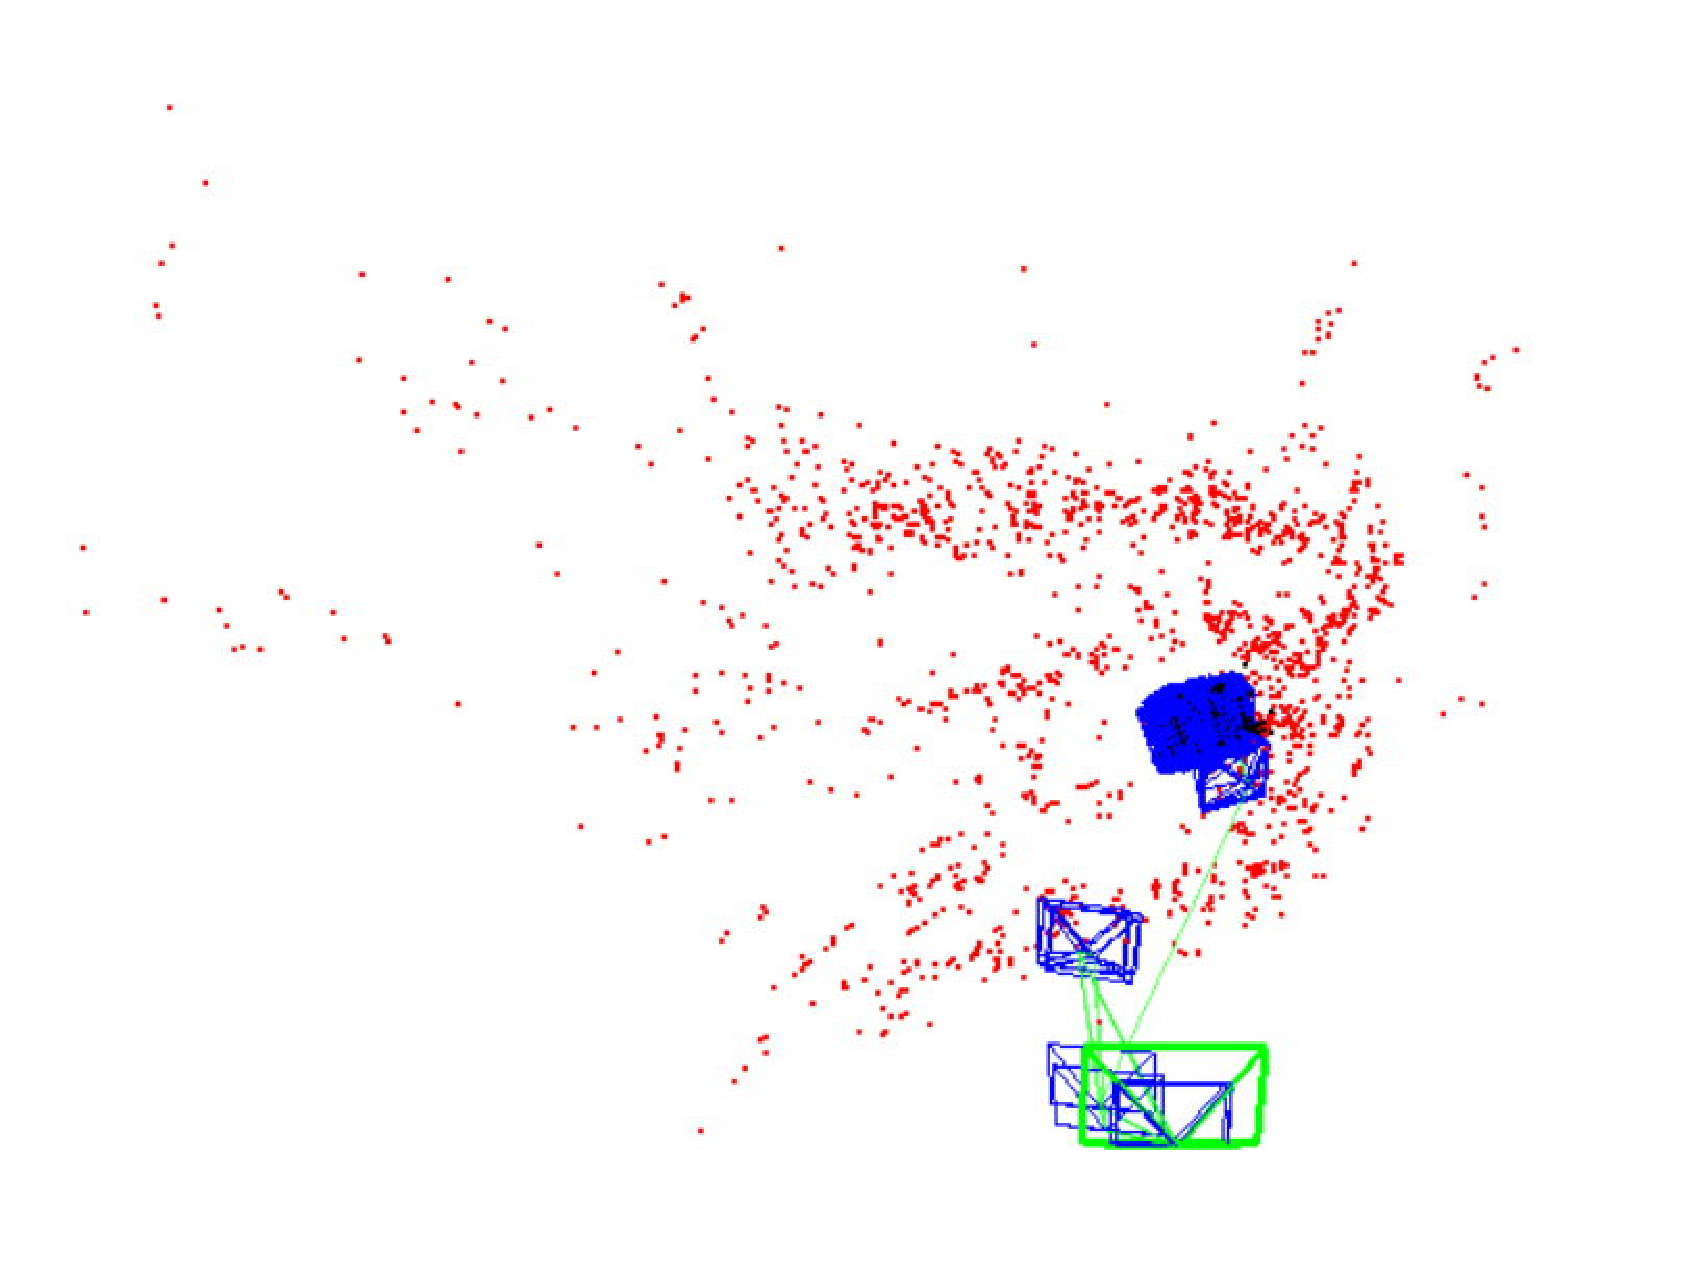
\includegraphics[width=10cm]{ORBSLAM2.pdf}
\caption{ORB-SLAM实际稀疏三维重建示意}
\label{fig:ORBSLAM3}
\end{figure}


\section{ORB-SLAM方法在家具设计与增强现实中的应用构想}
知名家居公司宜家(Ikra)于2014年推出了增强现实app,可以通过扫描目录页,而后把产品目录放在想要摆放家具的位置上,而后就可以在自己的手机或者平板电脑的屏幕上看到用户想要看到的家具放在自己家里的模样,其效果图如\autoref*{fig:yijia_app}所示。这种把家具拉出来与实际的居家环境结合的增强现实技术,带给了使用者更好的购物体验,而这也给宜家带来了巨大的收益。

\begin{figure}[!htbp]
\centering
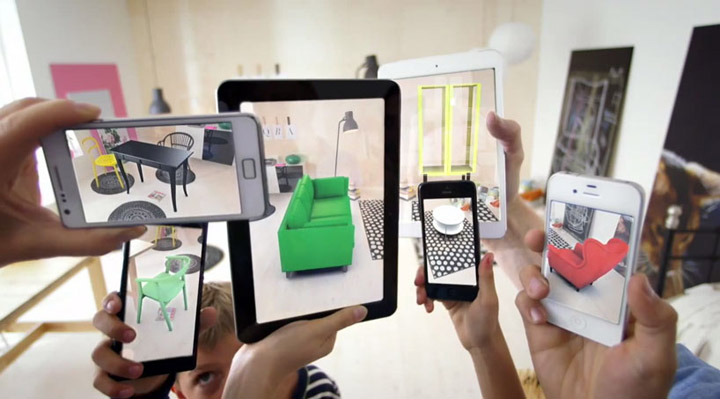
\includegraphics[width=12cm]{yijia_app.jpg}
\caption{Ikra app示意图}
\label{fig:yijia_app}
\end{figure}

然而,这个app有一个很大的缺点,那就是使用这个app需要购买宜家公司的产品目录,而其app采用的同时定位与地图构建方法则通过直接使用产品目录的位置大大简化了流程,即不再需要跟踪寻找关键帧,只需要跟踪产品目录的位置即可。这一行为于宜家公司来说绑定了产品目录的销量,另一方面却给用户带来了很多不便。

因此我们需要创造一个不需绑定产品目录,也能采用增强现实技术呈现家具在现实位置中摆放场景的app,这种app无疑能给客户带来更好的用户体验,那么,这个app的核心目标便是:跟踪,确定平面,渲染家具。

于是,我们期待能做到这样的一种增强现实app,app内可以从云端的家具模型库更新家具模型,存储在app内,而后,对于每一个场景,我们从手机的单目摄像头内读取场景的位置信息,对手机进行一个短距离的平移,而后调用ORB-SLAM算法,通过检测视差,得到两帧后,初始化Tracking-Mapping 双管线系统,而后再利用ORB-SLAM特有的loop closure模块消除误差,使得最大限度的得到现实场景的空间信息。而后用户可以将家具模型拖入手机屏幕的场景里,由于我们已经得到了现实场景的空间信息,因此我们可以在手机后台计算好家具的摆放位置,以及如何摆放才能使得家具在空间上显得更稳定,最后,再对家具模型进行场景渲染,针对摄像头获取的光线对家具的颜色、阴影进行渲染,使得在视觉上合理,用户从而获得更好的用户体验。

与宜家的app相比,这个app克服了产品目录与app使用上相互“绑定”的弊端,同时,从云端获取更新也方便商家随时更新自己的产品,而客户也可以第一时间获得商家最新的动态,同时,也可以嵌入商家的广告,不但从软广告——增强现实模拟方面,更从打硬广告获取用户的青睐。

相较于其他V-SLAM算法来说,ORB-SLAM误差小,速度快,可拓展性强,鲁棒性强,虽然依旧存在不少缺点(例如对于手机来说BA的效率和精度还是不够),但依旧存在着极高的应用前景及市场价值。

然而,实际运用当中,我们可能会遇到许多问题,例如,对于快速运动的物体,对物体的遮挡可能会导致物体暂时的丢失,即便ORB-SLAM相较于其他V-SLAM算法来说,可以迅速的找回物体,但也会给用户来带糟糕的用户体验,因此,在第四节中,我们将对ORB-SLAM算法进行一定的改进,使得ORB-SLAM可以较好地跟踪运动中的物体。